\section{Generative Adversarial Networks}
\label{sec:gan}

%%% when introduced, game theory approach
Generative Adversarial Networks (GAN) is a framework proposed in 2014 by Goodfellow et al. \cite{gan:2014} based on a game theoretic approach to generative modeling.
%which has gathered a lot of attention in the deep learning community and in the last few years many extensions have been [proposed] (citations).

GANs circumvent the issues arising around the inference problem by playing a two-player game. Both players play non-cooperatively against each other, which means they only try to maximize their respective success.
One player is called the generator $G$ which tries to produce authentic looking data samples while the other player, the discrimininator $D$ has to decide whether a received sample is generated or actually real data.
It is important to note that the generator gets to know whether the discriminator accepted the generated output as \emph{real} or rejected it as \emph{fake}.

As each party plays to maximize its own success, the discriminator will try to maximize the number of samples which got discriminated correctly.
On the other side, the generator tries to produce samples aiming to fool the discriminator.

As the game progresses, both parties will get better at their respective objective and the generated samples will look more and more like the training examples which is the ultimative goal is generative modeling.\\

%Using the analogy of counterfeiters and police can help understand the intuition behind game between $G$ and $D$ better.
%Counterfeiters will try to produce fake money looking to fool the police into thinking it is real money.
%The police however is able to distinguish badly made fake money from real money easily and as such rejects the fake money with high confidence.
%This rejection in turn triggers the counterfeiters to improve their forgery process try to imitate real money even better. Thus they are able to improve the quality of the faked money. Improvements made to the fake money in this iteration will lead to lower confidence with which the police is able to reject forgeries.


\paragraph{Solution}
The game-theoretic solution to the emerging situation where neither $G$ nor $D$ can improve its own success with respect to the outcome of the game gets called \emph{Nash equilibrium}\cite{game_theory:1994}.
In the case of GANs, this situation arises when the generator produces samples which get rejected with probability $p=0.5$ by the discriminator. In the case of such equilibrium, the generator produces good enough samples to fool the generator in about half cases.\\\\
\todo[inline]{Add some text showing the theoretical foundation of GANs}



Another formulation of the same game is to define the zero-sum game between the generative model and its adversary, the discriminator.
The payoff of the discriminator can be described as the value function $V(G,D)$ while the payoff of the generator is the negative payoff of $D$: $-V(G,D)$.\\
This formulation allows us to define the reached nash equlibium in equation \ref{eq:zerosum_convergence}.
\begin{equation}
  \label{eq:zerosum_convergence}
  G^* = \arg \min_{G} \max_{D} V(G,D)
\end{equation}


% use of words: forgery
%To understand the inuition behind the approach to GANs, it may be helpful to view(?) analogy of counterfeiters and the police.
%Counterfeiters try to produce fake money imitating legit money while the police tries to distinguish fake from real money.
%This procedure of generating and distinguishing will go back-and-forth as the counterfeiters will get better at producing authentic looking money and the police is hard-pressed to differentiate between fake and real.
%Eventually, this procedure will result in a nash equlibrium where the police or discriminator will have 50\% chance of seperating authentic from real.

%Ideally, we want to find this equilibrium for the GAN model as well.




%GANs can be understood as a two-player game where one player is called generator $G$ playing against the discriminator $D$.
%The goal of $G$ is to produce similar data to the given training set while $D$ is tasked with discriminating(?) the generated samples from the training data. Both $G$ and $D$ are learning function approximators, for example Multi-Layer Peceptron (MLP) networks as proposed in the original GAN paper.
% --> declare distribution p_data, p_model, x, z
%During learning, both networks are updated in parallel according to the gradient of their respective loss function which we will explore now.\\
%In the following $p_{data}$ is the true data generating distribution from which the training samples have been generated.
%We don't have access to that distribution.


\begin{figure}[htb]
\centering
\includestandalone[width=\textwidth,mode=buildnew]{media/gan_conceptual}
  \caption[GAN Architecture]{Architecture used for generative adversarial networks}
  \label{fig:gan_a}
  \medskip
  \small
  The above figure illustrates the computational graph and gradient flow in the GAN framework.\\
  $X$ denotes the dataset containing real-world data sampled from $p_{data}$, which we aim to model.\\
  Solid arrows indicate the forward pass in the model while dashed arrows denote the gradient flow during a backward pass.
\end{figure}

%\newpage

\subsection{Architecture}
\label{sub:gan_arch}
To formalize the setting in which the game between $G$ and $D$ takes place, we define the true, however unknown data distribution $p_{data}(x)$ from which samples are available as dataset $X=\{x^{(1)}, x^{(2)}, \dots, x^{(N)}\}$.

In the case of generative modeling, the goal is to approximate $p_{data}(x)$ with $p_{model}(x)$.
GANs uses neural network as function approximator for $G$ as well as $D$.
The generator network $G$ produces samples from $p_{model}(x)$ by transforming samples $z$ from random noise as $x = G(z)$.\\
Competing with $G$ is the discriminator $D$ trained to distinguish samples $ \tilde{x} \sim p_{model}(x)$ from real data $x \sim p_{data}(x)$.\\
Figure \ref{fig:gan_a} summarizes the described architecture with the respective gradient flow used to update $G$ and $D$.\\
%Formalizing the setup in a probabilistic way, we have the unknown data distribution $p_{data}(x)$ from which the training examples have been drawn and the marginalized model distribution $p_{model}(x) = \int p(z)p(x|z) \textit{d}z$ over the noise space $z$ (also latent space).


% http://www.slideshare.net/xavigiro/deep-learning-for-computer-vision-generative-models-and-adversarial-training-upc-2016
% TODO: recreate in tikz


%\begin{figure}[htb]
%\centering
%\includestandalone[mode=buildnew,width=\linewidth]{media/gan_conceptual}
  %\caption{Conceptual idea of generative adversarial networks (source: Summer seminar UPC TelecomBCN)}\label{fig:gan_architecture}
%\end{figure}


\subsubsection{Generator Network}
The generator $G$ in the GAN framework tries to fool the discriminator $D$ by producing samples which are indistinguishable from training data.
This process can formally be written as minimizing $\mathcal{L}_g$ in equation \ref{eq:l_g_1}.
%Where $z$ is sampling from the noise prior $p(z)$.\\

%Another common form of the generator loss is $\mathcal{L'}_g$.
%$$
\begin{equation}
  \label{eq:l_g_1}
  \mathcal{L}_g = \min \log\bigg(1 - D(G(z))\bigg)
\end{equation}

However, for gradient-based learning $\mathcal{L}_g$ provides poor gradient during learning \todo[inline]{early in training! show difference.} where the discriminator is able to reject samples from the generator with high confidence.\\
Therefore is equation \ref{eq:l_g_2} more commonly used in practice \todo[inline]{citations! dcgan? improved gan?}.

\begin{equation}
  \label{eq:l_g_2}
  \mathcal{L'}_g = \max \log D(G(z))
\end{equation}

Note that this loss function is fully differentiable which means it can be trained with backpropagation.



\subsubsection{Discriminator Network}
The objective of the discriminator network $D$ is to distinguish the generated samples produced by $G$ from the training set samples.
This process can be formalized to maximizing the cost function $\mathcal{L}_d$ in equation \ref{eq:l_d}.
\begin{equation}
  \label{eq:l_d}
  \mathcal{L}_d = \max \log\big(\log D(x) + \log (1 - D(G(z))\big)
\end{equation}



\subsection{Training}
\label{sub:gan_training}

\begin{figure}[htb]
\centering
  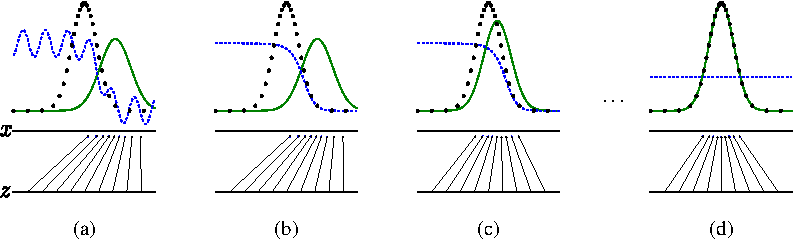
\includegraphics[width=\linewidth]{media/gan_training-crop}
  \caption[Learning Procedure in a GAN]{Learning a GAN on a one-dimensional distribution from the original paper\cite{gan:2014}}
  \label{fig:gan_training}
  \medskip
  \small
  The line named $z$ denotes the noise prior, while the arrows to the line indicated by $x$ is the transformation learned by the generator network. Three different distributions are showed, the solid line represents the generated sample in each step, while the dots are sampled from the data distribution $p_{data}(x)$. The dashed line shows the decision boundary with which probability the discriminator can distinguish between real and fake data.\\
  (a) Prior to training when both $D$ and $G$ are poor and $p_{model}$ does not match $p_{data}$.\\
  (b) After a step of learning $D$ with fixed $G$, the discriminator is able to distinguish fake from real samples easily as indicated by the decision boundary.\\
  (c) After a step of learning $G$ with fixed $D$ has the generator learned to produce samples more similar to $p_{data}(x)$.\\
  (d) The model has reached the nash equilibrium where $p_{model} = p_{data}$ and the discriminator can only distinguish between real and fake sample with $p=0.5$.
\end{figure}


Combining the two objectives into one value function yields equation \ref{eq:minimax_value} which is used to define minmax-game played by the two networks.
\begin{equation}
\label{eq:minimax_value}
\min_G \max_D V(D,G) = \mathbb{E}_{x \sim p_{data}}[\log D(x)] + \mathbb{E}_{z \sim p_z(z)}[\log(1 - D(G(z)))]
\end{equation}

The GAN framework can be fully trained with stochastic backpropagation due to $V(G,D)$ being differentiable with $G$ and $D$ implemented as (deep) neural nets.
Figure \ref{fig:gan_training} illustrates the ideal training procedure for learning of an one-dimensional distribution.
Training will switch between training the generator and discriminator, where the other party is fixed respectively.

%\paragraph{Theoretical Foundation}
Using a model with infinite training time as well as infinite capacity in both generator and discriminator allows to formulate the nash equilibrium in the generative adversarial network.
For any given generator $G$ and data points $x \sim p_{data}(x)$, the optimal discriminator $D$ is given by equation \ref{eq:opt_d}.
\begin{equation}
  \label{eq:opt_d}
  D_G^*(x) = \frac{p_{data}(x)}{p_{data}(x) + p_{model}(x)}
\end{equation}

%In the original GAN paper an minibatch-based algorithm for training GAN is proposed, but we will take a look at an the online learning version below:\\
%\begin{algorithm}
  %\caption{Online learning of generative adversarial networks $-$ simple version ($k=1$)}
  %\label{alg:gan_online}
  %\begin{algorithmic}[1]
    %\Let{$\eta_d, \eta_g$}{Learning rate of discriminator and generator networks, respectively}
    %\Let{$\theta_d, \theta_g$}{Parameters of function approximators}
    %\For{number of training iterations}
      %\Let{$z_d$}{sample from noise prior $p_g(z)$}
      %\Let{$z_g$}{sample from noise prior $p_g(z)$}
      %\Let{$x$}{example from training set}
      %\Let{$\theta_d$}{$\theta_d + \eta_d \nabla_{\theta_d} \bigg[\log D(x) + \log \big(1 - D(G(z_d))\big)\bigg]$}
      %\Let{$\theta_g$}{$\theta_g - \eta_g \nabla_{\theta_g} \bigg[\log\big(1 - D(G(z_d))\big)\bigg]$}
    %\EndFor
  %\end{algorithmic}
%\end{algorithm}

%In algorithm \ref{alg:gan_online} the original algorithm has been modified for single pass (online) learning.
%Sampling minibatches from the noise prior and $p_{data}(x)$ result in the minibatch version.
%Additionally, it is often required for practical reasons to let the discriminator run multiple backward passes while updating the generator once (why?).
%Note that the discriminator will ascend while the generator descend its gradient due to maximizing $\mathcal{L}_d$ but minimizing $\mathcal{L}_g$ (correct?).

\newpage

\subsection{Stability and Performance}
\label{sub:gan_stability}
In the common case where both function approximators $G$ and $D$ are implemented using deep neural networks, GANs have been shown to be difficult to train using gradient descent.
In fact, there is no guarantee that GANs will converge in the case of using non-convex functions to represent $G$ or $D$.

%These issues have been credited to the problem of finding the nash equilibrium in the minimax-game with continious, high-dimensional parameters instead of more traditional optimization problems.
%TheseAdditionally to these hypothetical thoughts, \cite{gan_distinguish_crit:2014} have shown that these methods may fail to converge.
Acknowledging these problems, Salimans et al.\cite{improved_gan:2016} has studied the stability and performance of GAN in detail, resulting in a number of practical methods improving performance of the training procedure of GANs.
We will take a look at a selection of these methods in the following, focussing on deep neural networks as approximators in both $D$ and $G$.

\subsubsection{Freeze Learning}
\label{ssub:gan_freeze_learning}
One of the main issues prominent during GAN training is the disparity in performance between $G$ and $D$.
Most of the time during training will one network outperform the other player by such great margin that the gradients from the stronger player will vanish resulting in even slower training for the weaker network.
Thus one of the common practices\cite{improved_gan:2016}\cite{dcgan:2015} for learning GANs is to freeze one network and prevent it from learning until the other player has catched up.
%In practice the generator is far slower to train than the discriminator in most cases (citation).


\subsubsection{Label Smoothing \cite{improved_gan:2016}}
\label{ssub:gan_label_smoothing}
Another rather basic idea to improve gradient flow is to replace the binary classification from the discriminator with smoothed values $0.1/0.9$ or $\epsilon/1-\epsilon$.
This helps the generator with an informative gradient to improve learning performance.
Additionally, smoothed labels have been shown to reduce the attack surface of neural networks to adversarial examples \cite{adv_examples:2016}.
% TODO replace 0/1 with e/1 − e ??
% TODO one-sided label smoothing


\subsubsection{(Virtual) Batch normalization}
\label{ssub:gan_batch_norm}
% TODO explain internal covariate shift?
Batch normalization (BN) \cite{batch_norm:2015} is a recent technique to boost performance in deep neural networks addressing the \emph{internal covariate shift} by normalizing minibatches.
Essentially, BN works by normalizing each sample from a minibatch to the statistics of the whole batch.
To improve training performance of GANs, a modified version of batch normalization has been proposed \cite{improved_gan:2016} for training of the generator.
Instead of normalizing each input $x$ to their corresponding minibatch, one reference batch is chosen prior to training which will be used to normalize all further input.

%In a paper \cite{improved_gan:2016} by Salimans et al on improving stability of the GAN training procedure, a variant of BN has been proposed called virtual batch normalization.


%Using batch normalization \cite{batch_norm:2015} helped stabilizing learning DCGAN \cite{dcgan:2015}.
%\cite{improved_gan:2016} introduced virtual batch normalization where each input $x$ is normalized on one reference batch chosen at the start of learning instead of the other inputs in the mini-batch.

\subsubsection{Feature Matching}
\label{ssub:gan_feature_matching}
In computer vision, features are often used to identify relevant pieces of information in images for recognition and classification.
They may refer to a set of points or edges in an image, which exactly is not clearly defined.
With the recent advances in classification tasks performed by deep convolutional networks, automatically learned features have been a large part of that success.
Feature matching is an technique designed to improve the learning procedure of GANs where not directly $\mathcal{L}_g$ is maximized but instead also learn the discriminator on intermediate layer activation outputs.
Using this modified procedure aids the generator to output data matching the statistics of the input data more closely.
%With $f(x)$ denoting an intermediate layer in $D$, the new objective function becomes:
%$$
%|| \mathbb{E}_{x \sim p_{data}}f(x) - \mathbb{E}_{z \sim p(z)}f(G(z)) || ^{2}_{2}
%$$




%\subsection{Application}
%\label{sub:gan_application}
%GAN have been applied to many different areas which include generating images (GAN, DCGAN, LAPGAN), sequences (SeqGAN), videos (\cite{gan_video:2016}), 3D objects (\cite{gan_3d:2016}), text-to-image synthesis (\cite{gan_t2i:2016})


\subsection{Extensions}
\label{sub:gan_extensions}

\subsubsection{Deep Convolutional GAN}
\label{ssub:dcgan}
Deep convolutional networks\cite{lecun-89e} have yielded impressive results for image classification \cite{imagenet:2012} and have arguably been one of the main reasons for the recent success of deep learning.
These techniques however have mostly been applied in a supervised learning context, not with unsupervised learning.

The discriminator in the GAN model implements a binary classification task and the performance of the generator is heavily dependent on the discriminator, as the training procedure uses the discriminator in the objective function $\mathcal{L}_{g}$ in equation \ref{eq:l_g_1} and \ref{eq:l_g_2}.\\
This leads to the suggestion that using deep convolutional networks helps boost the model performance. In fact is the deep convolution GAN proposed by Radford et al.\cite{dcgan:2015} one of the first GAN variants which results in visually pleasing results.

In order to use convolutional networks in the generator and discriminator, fractionally strided convolutions have been used to basically upsample the image. The exact details of the architecture is beyond the scope of this article, however in addition to the impressive generative performance the authors have shown that the model has learned to produce representional structures in latent space.
Furthermore, as shown in Figure \ref{fig:dcgan_vector} they were able to perform vector artithmetic in the latent space with results indicating that their model was able to arrange the latent space in a useful way.
\todo[inline]{Elaborate on how DCGAN arranges latent space}

\begin{figure}[t]
\centering
  \includegraphics[width=\linewidth]{media/dcgan_vector}
  \caption[Vector arithmetic in DCGAN]{Vector arithmetic performed in latent space $z$, from DCGAN paper\cite{dcgan:2015}}
  \label{fig:dcgan_vector}
  \medskip
  \small
\end{figure}

\newpage
\subsubsection{Laplacian Generative Adversarial Networks}
\label{ssub:lapgan}
%Applied to unsupervised learning in the case of GANs, deep convolutional GANs (DCGAN\cite{dcgan:2015}) has shown great success in producing images with 

%Early implementations of the GAN framework have been implemented using fully-connected layers,
%which have proven to be difficult and slow to train on real-world data (citation, original convnet papers?).
%Using deep convolutional networks has helped reach human-level performance in object recognition and classification problems on images (citations!).
%\emph{Deep convolutional generative adversarial network} (DCGAN) has applied convolutional networks to both generator and discriminator, resulting in quantitively evualuated better results.
%DCGAN uses no fully connected or pooling layers, but instead fractionally strided convolutions (often wrongfully called deconvolutions).

\begin{figure}[t]
\centering
  \includegraphics[width=\linewidth]{media/bedroom_scenes-crop}
  \caption[Generated Samples by DCGAN]{Bedroom scenes generated by the DCGAN model, from the original paper\cite{lapgan:2015}}
  \label{fig:lapgan}
  \medskip
  \small
\end{figure}
Laplacian Generative Adversarial Networks (LAPGAN) \cite{lapgan:2015} are an extension to GANs applied to images using laplacian pyramids \cite{laplacian:1983}.
Instead of using a single generator network, LAPGAN uses a series of deep convolutional networks as generators where each generator receives the output of the previous generator.




\paragraph{Training} is heavily modified from the regular GAN framework.
In each iteration a training sample is drawn from the dataset and a downsamples version from it is computed.
The discriminator receives now either the computed high-pass image (from the original image and the down-then-up sampled image) or an high-pass image from the generator.
These steps are repeated for other steps, downscaling the image.
In the last stage, a traditional generator and discriminator is used for the $8\times8$ image.
\paragraph{Sampling} uses a conditional GAN to produce high-resolution images through different stages of deep generator networks.

\paragraph{Results}
As GANs have no direct measurement of the quality of generations due to their lack of unified objective function, human evaluation of the authenticity of generated images is often used for qualitively evaluation.
LAPGAN has pushed the state of the art significantly, with generated images which are high-resolution in comparison to earlier methods and arguably high variety of generated images as shown in Figure \ref{fig:lapgan}.
Furthermore, humans have mistaken the generated images for real images 40\% of the time.


